\chapter{A meiose e o embaralhamento genético}\label{ch:g12:meiosis-genetic-shuffling}

Dois pais, cada um com 46 \omterm{def:g10:universal-dna:information}{cromossomos}, produzem um filho com 46 --- e
não 92. Em algum ponto entre os corpos dos pais e o filho, a contagem é
dividida pela metade, e é dividida de um jeito que dá a cada filho uma
mão que nenhum irmão jamais teve: os mesmos pais, quarenta anos de
filhos, e nenhum par igual, exceto os gêmeos idênticos. A divisão pela
metade é uma divisão especial chamada \omterm{def:g12:meiosis-genetic-shuffling:meiosis}{meiose}; a distribuição das cartas
é o que ela faz com os \omterm{def:g10:universal-dna:information}{cromossomos} pelo caminho. Este capítulo
acompanha uma \omterm{def:g10:cells-common-unit:cell}{célula} ao longo da \omterm{def:g12:meiosis-genetic-shuffling:meiosis}{meiose}, conta as combinações que ela
pode produzir, e lê os resultados de cruzamentos que revelam, de fora,
o que aconteceu por dentro.

\section{Dividir o conjunto pela metade}

\begin{definition}[Diploide, haploide, meiose]\label{def:g12:meiosis-genetic-shuffling:meiosis}
Uma \omterm{def:g10:cells-common-unit:cell}{célula} que carrega duas cópias de cada \omterm{def:g11:cell-cycle-mitosis:chromosome}{cromossomo} --- uma de cada
genitor, formando as duas um par de \emph{\omterm{def:g10:universal-dna:information}{cromossomos} homólogos} --- é
\emph{diploide}\index{diploide}, escrito $2n$ ($2n = 46$ nos seres
humanos). Uma \omterm{def:g10:cells-common-unit:cell}{célula} que carrega uma cópia de cada é
\emph{haploide}\index{haploide}, escrito $n$. A
\emph{meiose}\index{meiose} é a sequência de duas divisões pela qual
uma \omterm{def:g10:cells-common-unit:cell}{célula} diploide, depois de uma única \omterm{def:g11:dna-replication:replication}{replicação do DNA} dela,
produz quatro \omterm{def:g10:cells-common-unit:cell}{células} haploides --- os gametas, ou as precursoras
deles. A \emph{fecundação} une dois gametas haploides e restaura o
número diploide: a alternância de meiose e fecundação é o ciclo de toda
\omterm{def:g10:biodiversity-scales:species}{espécie} que se reproduz sexuadamente.
\end{definition}

\begin{proposition}[As duas divisões]\label{prop:g12:meiosis-genetic-shuffling:divisions}
Antes da \omterm{def:g12:meiosis-genetic-shuffling:meiosis}{meiose} o \omterm{def:g10:universal-dna:information}{DNA} é replicado: cada \omterm{def:g11:cell-cycle-mitosis:chromosome}{cromossomo} tem duas
\omterm{def:g11:cell-cycle-mitosis:chromosome}{cromátides}. Depois:
\begin{itemize}
  \item \emph{Primeira divisão} (\omterm{def:g12:meiosis-genetic-shuffling:meiosis}{meiose} I, \emph{reducional}): os
        \omterm{def:g10:universal-dna:information}{cromossomos} homólogos se emparelham, dois a dois, no equador;
        os membros de cada par são puxados para polos opostos. Cada
        célula-filha recebe \emph{um \omterm{def:g11:cell-cycle-mitosis:chromosome}{cromossomo} de cada par}, ainda
        formado por duas \omterm{def:g11:cell-cycle-mitosis:chromosome}{cromátides}: $n$ \omterm{def:g10:universal-dna:information}{cromossomos}, quantidade de
        \omterm{def:g10:universal-dna:information}{DNA} $q$ (a quantidade de uma \omterm{def:g10:cells-common-unit:cell}{célula} \omterm{def:g12:meiosis-genetic-shuffling:meiosis}{diploide} antes da
        replicação).
  \item \emph{Segunda divisão} (\omterm{def:g12:meiosis-genetic-shuffling:meiosis}{meiose} II, \emph{equacional}): como
        numa \omterm{def:g11:cell-cycle-mitosis:cycle}{mitose}, as \omterm{def:g11:cell-cycle-mitosis:chromosome}{cromátides} de cada \omterm{def:g11:cell-cycle-mitosis:chromosome}{cromossomo} se separam. Cada
        uma das quatro \omterm{def:g10:cells-common-unit:cell}{células} recebe $n$ \omterm{def:g10:universal-dna:information}{cromossomos} de uma \omterm{def:g11:cell-cycle-mitosis:chromosome}{cromátide},
        quantidade de \omterm{def:g10:universal-dna:information}{DNA} $q/2$.
\end{itemize}
A primeira divisão divide pela metade o número de \omterm{def:g10:universal-dna:information}{cromossomos}; a
segunda divide pela metade a quantidade de \omterm{def:g10:universal-dna:information}{DNA}, voltando a uma
\omterm{def:g11:cell-cycle-mitosis:chromosome}{cromátide} por \omterm{def:g11:cell-cycle-mitosis:chromosome}{cromossomo}.
\end{proposition}
\admitted

\begin{omfigure}
\begin{tikzpicture}[font=\small, line cap=round]
  \tikzset{cellb/.style={draw, thick, fill=omDef!5, rounded corners=9pt, minimum width=2.5cm, minimum height=2.5cm},
           ma/.style={line width=3pt, omDef!80}, mb/.style={line width=3pt, omThm!80},
           mA/.style={line width=3pt, omDef!35}, mB/.style={line width=3pt, omThm!35}, cen/.style={fill=black}}
  % panel 1: diploid cell after S: two pairs (long pair blue, short pair red); paternal dark, maternal pale
  \begin{scope}
    \node[cellb] at (0,0) {};
    \draw[ma] (-0.75,0.7) .. controls (-0.62,0.1) .. (-0.75,-0.5); \draw[ma] (-0.49,0.7) .. controls (-0.62,0.1) .. (-0.49,-0.5); \fill[cen] (-0.62,0.1) circle (1.6pt);
    \draw[mA] (-0.2,0.7) .. controls (-0.07,0.1) .. (-0.2,-0.5); \draw[mA] (0.06,0.7) .. controls (-0.07,0.1) .. (0.06,-0.5); \fill[cen] (-0.07,0.1) circle (1.6pt);
    \draw[mb] (0.4,0.45) .. controls (0.53,0.1) .. (0.4,-0.25); \draw[mb] (0.66,0.45) .. controls (0.53,0.1) .. (0.66,-0.25); \fill[cen] (0.53,0.1) circle (1.6pt);
    \draw[mB] (0.9,0.45) .. controls (1.03,0.1) .. (0.9,-0.25); \draw[mB] (1.16,0.45) .. controls (1.03,0.1) .. (1.16,-0.25); \fill[cen] (1.03,0.1) circle (1.6pt);
    \node[anchor=north, align=center, font=\scriptsize, text width=3.05cm] at (0,-1.35) {depois da replicação:\\ $2n = 4$, DNA $2q$};
  \end{scope}
  % panel 2: metaphase I: pairs on the equator
  \begin{scope}[xshift=3.2cm]
    \node[cellb] at (0,0) {};
    \draw[dashed, gray] (-1.1,0) -- (1.1,0);
    \draw[ma] (-0.7,0.55) .. controls (-0.57,0.1) .. (-0.7,-0.35); \draw[ma] (-0.44,0.55) .. controls (-0.57,0.1) .. (-0.44,-0.35); \fill[cen] (-0.57,0.15) circle (1.6pt);
    \draw[mA] (-0.7,-0.05) .. controls (-0.57,-0.5) .. (-0.7,-0.95); \draw[mA] (-0.44,-0.05) .. controls (-0.57,-0.5) .. (-0.44,-0.95); \fill[cen] (-0.57,-0.15) circle (1.6pt);
    \draw[mb] (0.45,0.5) .. controls (0.58,0.2) .. (0.45,-0.1); \draw[mb] (0.71,0.5) .. controls (0.58,0.2) .. (0.71,-0.1); \fill[cen] (0.58,0.15) circle (1.6pt);
    \draw[mB] (0.45,0.1) .. controls (0.58,-0.2) .. (0.45,-0.5); \draw[mB] (0.71,0.1) .. controls (0.58,-0.2) .. (0.71,-0.5); \fill[cen] (0.58,-0.15) circle (1.6pt);
    \node[anchor=north, align=center, font=\scriptsize, text width=3.05cm] at (0,-1.35) {meiose I: pares de\\ homólogos no equador};
  \end{scope}
  % panel 3: two cells after MI, each n=2 with two chromatids
  \begin{scope}[xshift=6.4cm]
    \node[cellb, minimum height=1.15cm] at (0,0.7) {};
    \node[cellb, minimum height=1.15cm] at (0,-0.7) {};
    \draw[ma] (-0.55,1.15) .. controls (-0.42,0.7) .. (-0.55,0.25); \draw[ma] (-0.29,1.15) .. controls (-0.42,0.7) .. (-0.29,0.25); \fill[cen] (-0.42,0.7) circle (1.6pt);
    \draw[mB] (0.35,1.0) .. controls (0.48,0.7) .. (0.35,0.4); \draw[mB] (0.61,1.0) .. controls (0.48,0.7) .. (0.61,0.4); \fill[cen] (0.48,0.7) circle (1.6pt);
    \draw[mA] (-0.55,-0.25) .. controls (-0.42,-0.7) .. (-0.55,-1.15); \draw[mA] (-0.29,-0.25) .. controls (-0.42,-0.7) .. (-0.29,-1.15); \fill[cen] (-0.42,-0.7) circle (1.6pt);
    \draw[mb] (0.35,-0.4) .. controls (0.48,-0.7) .. (0.35,-1.0); \draw[mb] (0.61,-0.4) .. controls (0.48,-0.7) .. (0.61,-1.0); \fill[cen] (0.48,-0.7) circle (1.6pt);
    \node[anchor=north, align=center, font=\scriptsize, text width=3.05cm] at (0,-1.35) {duas células: $n = 2$,\\ duas cromátides, DNA $q$};
  \end{scope}
  % panel 4: four cells after MII, single chromatids
  \begin{scope}[xshift=9.6cm]
    \foreach \y in {1.05,0.35,-0.35,-1.05} \node[cellb, minimum height=0.6cm, minimum width=2.3cm] at (0,\y) {};
    \draw[ma] (-0.5,1.3) -- (-0.5,0.8); \fill[cen] (-0.5,1.05) circle (1.4pt); \draw[mB] (0.4,1.22) -- (0.4,0.88); \fill[cen] (0.4,1.05) circle (1.4pt);
    \draw[ma] (-0.5,0.6) -- (-0.5,0.1); \fill[cen] (-0.5,0.35) circle (1.4pt); \draw[mB] (0.4,0.52) -- (0.4,0.18); \fill[cen] (0.4,0.35) circle (1.4pt);
    \draw[mA] (-0.5,-0.1) -- (-0.5,-0.6); \fill[cen] (-0.5,-0.35) circle (1.4pt); \draw[mb] (0.4,-0.18) -- (0.4,-0.52); \fill[cen] (0.4,-0.35) circle (1.4pt);
    \draw[mA] (-0.5,-0.8) -- (-0.5,-1.3); \fill[cen] (-0.5,-1.05) circle (1.4pt); \draw[mb] (0.4,-0.88) -- (0.4,-1.22); \fill[cen] (0.4,-1.05) circle (1.4pt);
    \node[anchor=north, align=center, font=\scriptsize, text width=3.05cm] at (0,-1.45) {quatro gametas: $n = 2$,\\ uma cromátide, DNA $q/2$};
  \end{scope}
\end{tikzpicture}

{\small A \omterm{def:g12:meiosis-genetic-shuffling:meiosis}{meiose} numa \omterm{def:g10:cells-common-unit:cell}{célula} com dois pares de \omterm{def:g10:universal-dna:information}{cromossomos} ($2n = 4$);
os tons escuros e claros marcam os dois membros de cada par, vindos dos
dois genitores. A primeira divisão separa os homólogos, a segunda as
\omterm{def:g11:cell-cycle-mitosis:chromosome}{cromátides}. Aqui o \omterm{def:g11:cell-cycle-mitosis:chromosome}{cromossomo} escuro comprido foi junto com o claro
curto: um dos dois arranjos possíveis.}
\end{omfigure}

\begin{omfigure}
\begin{tikzpicture}
\begin{axis}[
  width=0.88\linewidth, height=5.2cm,
  axis x line=bottom, axis y line=left,
  xmin=0, xmax=10, ymin=0, ymax=2.7,
  xlabel={tempo}, ylabel={DNA por célula},
  xlabel style={font=\small, at={(axis description cs:0.5,-0.1)}, anchor=north},
  ylabel style={font=\small},
  tick label style={font=\small}, xtick=\empty,
  ytick={0.5,1,2}, yticklabels={$q/2$, $q$, $2q$},
  clip=false,
]
\addplot[thick, omDef] coordinates {(0,1) (2,1) (4,2) (5.9,2) (6,1) (7.9,1) (8,0.5) (10,0.5)};
\draw[dashed, gray] (axis cs:2,0) -- (axis cs:2,2.2); \draw[dashed, gray] (axis cs:4,0) -- (axis cs:4,2.2);
\draw[dashed, gray] (axis cs:6,0) -- (axis cs:6,2.2); \draw[dashed, gray] (axis cs:8,0) -- (axis cs:8,2.2);
\node[font=\small, anchor=south] at (axis cs:1,2.25) {$2n$, $q$};
\node[font=\small, anchor=south] at (axis cs:3,2.25) {fase S};
\node[font=\small, anchor=south] at (axis cs:5,2.25) {$2n$, $2q$};
\node[font=\small, anchor=south, omThm] at (axis cs:6,2.45) {meiose I};
\node[font=\small, anchor=south] at (axis cs:7,2.25) {$n$, $q$};
\node[font=\small, anchor=south, omThm] at (axis cs:8,2.45) {meiose II};
\node[font=\small, anchor=south] at (axis cs:9,2.25) {$n$, $q/2$};
\end{axis}
\end{tikzpicture}

{\small O \omterm{def:g10:universal-dna:information}{DNA} por \omterm{def:g10:cells-common-unit:cell}{célula} ao longo da \omterm{def:g12:meiosis-genetic-shuffling:meiosis}{meiose}. Uma replicação, depois
duas divisões sem replicação entre elas: os gametas guardam um quarto
do \omterm{def:g10:universal-dna:information}{DNA} que a célula-mãe tinha depois de S, e metade do que uma \omterm{def:g10:cells-common-unit:cell}{célula}
\omterm{def:g12:meiosis-genetic-shuffling:meiosis}{diploide} tem em repouso.}
\end{omfigure}

\begin{example}[Os números humanos]\label{ex:g12:meiosis-genetic-shuffling:numbers}
Uma \omterm{def:g10:cells-common-unit:cell}{célula} germinativa do testículo, $2n = 46$, replica e fica com 46
\omterm{def:g10:universal-dna:information}{cromossomos} de duas \omterm{def:g11:cell-cycle-mitosis:chromosome}{cromátides} ($2q$); depois da \omterm{def:g12:meiosis-genetic-shuffling:meiosis}{meiose} I, duas \omterm{def:g10:cells-common-unit:cell}{células}
de 23 \omterm{def:g10:universal-dna:information}{cromossomos} de duas \omterm{def:g11:cell-cycle-mitosis:chromosome}{cromátides} ($q$); depois da \omterm{def:g12:meiosis-genetic-shuffling:meiosis}{meiose} II, quatro
espermatozoides de 23 \omterm{def:g10:universal-dna:information}{cromossomos} de uma \omterm{def:g11:cell-cycle-mitosis:chromosome}{cromátide} ($q/2$). Na
fecundação, $23 + 23 =
46$ e $q/2 + q/2 = q$: o zigoto volta a ser uma \omterm{def:g10:cells-common-unit:cell}{célula} \omterm{def:g12:meiosis-genetic-shuffling:meiosis}{diploide} em
repouso. No ovário, as mesmas divisões produzem um óvulo grande e três
\omterm{def:g10:cells-common-unit:cell}{células} minúsculas que são descartadas; a aritmética é idêntica.
\end{example}

\section{O embaralhamento}

\begin{proposition}[Segregação independente]\label{prop:g12:meiosis-genetic-shuffling:assortment}
Na metáfase I, cada par de homólogos se alinha no equador de modo
independente dos outros pares: qual membro de um par vai para qual polo
é decidido pelo acaso, par por par. Uma \omterm{def:g10:cells-common-unit:cell}{célula} com $n$ pares pode
produzir, portanto, $2^n$ combinações diferentes de \omterm{def:g10:universal-dna:information}{cromossomos}
paternos e maternos nos gametas dela --- $2^{23} \approx \num{8.4e6}$
num ser humano. A fecundação, ao unir ao acaso dois gametas desses,
rende $2^{23}
\times 2^{23} \approx \num{7e13}$ combinações de \omterm{def:g10:universal-dna:information}{cromossomos} para os
filhos de um casal, antes de qualquer outra fonte de variedade ser
contada.
\end{proposition}
\admitted

\begin{proposition}[A permutação]\label{prop:g12:meiosis-genetic-shuffling:crossingover}
Enquanto os homólogos estão emparelhados, no início da \omterm{def:g12:meiosis-genetic-shuffling:meiosis}{meiose} I, duas
\omterm{def:g11:cell-cycle-mitosis:chromosome}{cromátides} não irmãs se rompem no mesmo ponto e se reúnem em cruz: é
uma \emph{permutação}\index{permutação}. Cada \omterm{def:g11:cell-cycle-mitosis:chromosome}{cromátide} além do ponto
de troca passa a carregar os \omterm{def:g10:universal-dna:gene}{alelos} do outro homólogo. Os \omterm{def:g10:universal-dna:information}{cromossomos}
que chegam aos gametas não são, portanto, os \omterm{def:g10:universal-dna:information}{cromossomos} dos genitores,
e sim \omterm{def:g10:universal-dna:information}{cromossomos} \emph{recombinados}, que misturam ao longo do
comprimento deles os \omterm{def:g10:universal-dna:gene}{alelos} recebidos dos dois avós. Uma a três trocas
acontecem em cada par a cada \omterm{def:g12:meiosis-genetic-shuffling:meiosis}{meiose}, em posições variáveis: o número de
gametas possíveis é, na prática, ilimitado.
\end{proposition}
\begin{proof}[Evidências]
Ao microscópio, os homólogos emparelhados na \omterm{def:g12:meiosis-genetic-shuffling:meiosis}{meiose} I mostram pontos
cruzados, os \emph{quiasmas}, em que duas \omterm{def:g11:cell-cycle-mitosis:chromosome}{cromátides} visivelmente
trocam de parceira. Cruzamentos em que dois \omterm{def:g10:universal-dna:gene}{genes} ficam no mesmo
\omterm{def:g11:cell-cycle-mitosis:chromosome}{cromossomo} dão, entre os descendentes, uma minoria que carrega
combinações novas dos \omterm{def:g10:universal-dna:gene}{alelos} dos dois \omterm{def:g10:universal-dna:gene}{genes} --- combinações que nenhum
dos genitores carregava --- numa proporção que depende da distância
entre os \omterm{def:g10:universal-dna:gene}{genes}; \omterm{def:g10:universal-dna:gene}{genes} bem afastados num \omterm{def:g11:cell-cycle-mitosis:chromosome}{cromossomo} recombinam com a
mesma frequência que \omterm{def:g10:universal-dna:gene}{genes} de \omterm{def:g10:universal-dna:information}{cromossomos} diferentes. Marcadores
moleculares acompanhados ao longo das famílias mostram os segmentos de
cada \omterm{def:g11:cell-cycle-mitosis:chromosome}{cromossomo} trocando de origem avoenga em um ou dois pontos por
\omterm{def:g11:cell-cycle-mitosis:chromosome}{cromossomo} por geração.
\end{proof}

\begin{omfigure}
\begin{tikzpicture}[font=\small, line cap=round, >=Stealth]
  \tikzset{p/.style={line width=4pt, omDef!80}, m/.style={line width=4pt, omThm!70}}
  % before: two homologues, each two chromatids; alleles A/a, B/b
  \draw[p] (0,0) -- (0,3); \draw[p] (0.35,0) -- (0.35,3);
  \draw[m] (0.9,0) -- (0.9,3); \draw[m] (1.25,0) -- (1.25,3);
  \foreach \x in {0,0.35} { \node[font=\scriptsize, anchor=east, xshift=-1pt] at (\x,2.6) {}; }
  \node[font=\scriptsize, omDef!80!black, anchor=east] at (-0.15,2.6) {$A$};
  \node[font=\scriptsize, omDef!80!black, anchor=east] at (-0.15,0.5) {$B$};
  \node[font=\scriptsize, omThm!80!black, anchor=west] at (1.4,2.6) {$a$};
  \node[font=\scriptsize, omThm!80!black, anchor=west] at (1.4,0.5) {$b$};
  \node[anchor=north, align=center] at (0.62,-0.2) {homólogos emparelhados\\ (duas cromátides cada)};
  \draw[->, thick] (2.4,1.5) -- (3.4,1.5);
  % during: chiasma between the two inner chromatids at y=1.5
  \begin{scope}[xshift=4.2cm]
    \draw[p] (0,0) -- (0,3);
    \draw[p] (0.35,3) -- (0.35,1.6) -- (0.9,1.4) -- (0.9,0);
    \draw[m] (0.9,3) -- (0.9,1.6) -- (0.35,1.4) -- (0.35,0);
    \draw[m] (1.25,0) -- (1.25,3);
    \node[anchor=north, align=center] at (0.62,-0.2) {quiasma: duas cromátides\\ se rompem e se reúnem em cruz};
  \end{scope}
  \draw[->, thick] (6.6,1.5) -- (7.6,1.5);
  % after: four chromatids separated
  \begin{scope}[xshift=8.4cm]
    \draw[p] (0,0) -- (0,3);
    \draw[p] (0.5,3) -- (0.5,1.5); \draw[m] (0.5,1.5) -- (0.5,0);
    \draw[m] (1.0,3) -- (1.0,1.5); \draw[p] (1.0,1.5) -- (1.0,0);
    \draw[m] (1.5,0) -- (1.5,3);
    \node[font=\scriptsize, anchor=south] at (0,3.05) {$AB$};
    \node[font=\scriptsize, anchor=south] at (0.5,3.05) {$Ab$};
    \node[font=\scriptsize, anchor=south] at (1.0,3.05) {$aB$};
    \node[font=\scriptsize, anchor=south] at (1.5,3.05) {$ab$};
    \node[anchor=north, align=center] at (0.75,-0.2) {quatro gametas: dois parentais,\\ dois recombinados};
  \end{scope}
\end{tikzpicture}

{\small Uma \omterm{prop:g12:meiosis-genetic-shuffling:crossingover}{permutação} entre dois \omterm{def:g10:universal-dna:gene}{genes} $A$ e $B$ do mesmo \omterm{def:g11:cell-cycle-mitosis:chromosome}{cromossomo}.
Duas das quatro \omterm{def:g11:cell-cycle-mitosis:chromosome}{cromátides} trocam as extremidades delas; dos quatro
gametas, dois carregam as combinações parentais ($AB$, $ab$) e dois
carregam combinações novas ($Ab$, $aB$).}
\end{omfigure}

\begin{omfigure}
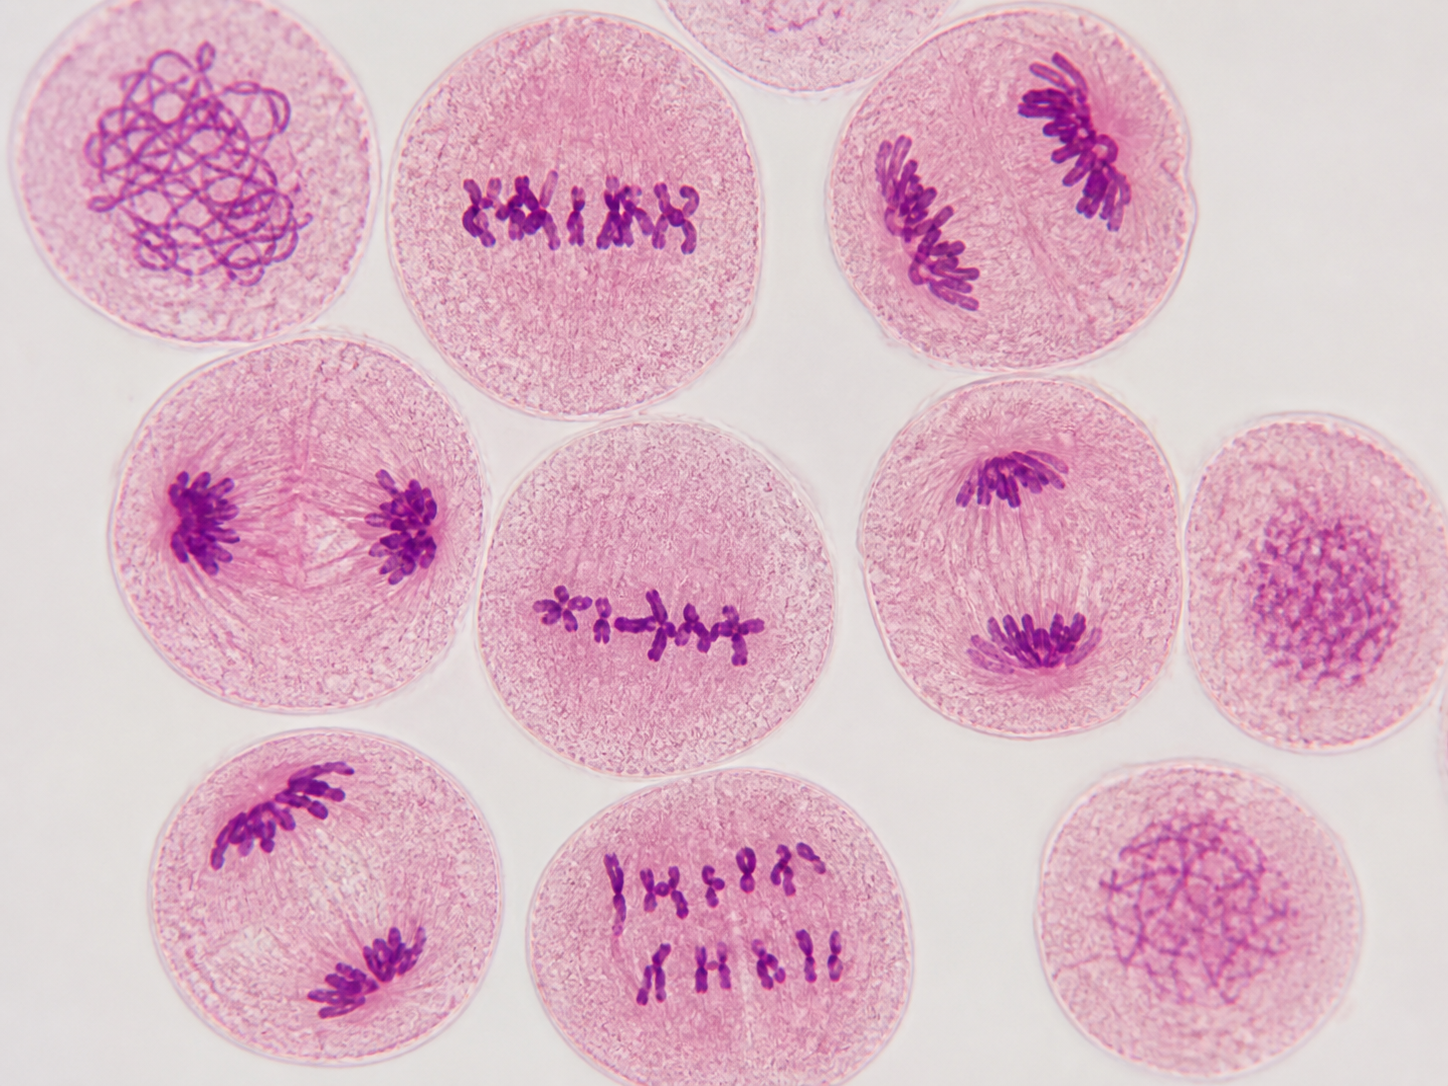
\includegraphics[width=0.56\linewidth]{images/book2/ai/g12-meiosis-lily-anther.png}

{\small \omterm{def:g10:cells-common-unit:cell}{Células} de uma antera de lírio em \omterm{def:g12:meiosis-genetic-shuffling:meiosis}{meiose}, coradas: em algumas,
os homólogos emparelhados se alinham no meio da \omterm{def:g10:cells-common-unit:cell}{célula}; em outras eles
já foram puxados para os dois polos. As etapas do esquema, vistas no
tecido que fabrica o pólen.}
\end{omfigure}

\begin{example}[Três fontes de variedade, em ordem]\label{ex:g12:meiosis-genetic-shuffling:sources}
Um filho de dois genitores é novo de três maneiras: a \omterm{prop:g12:meiosis-genetic-shuffling:crossingover}{permutação}
reconstruiu cada \omterm{def:g11:cell-cycle-mitosis:chromosome}{cromossomo} de cada gameta a partir das duas cópias
avoengas; a segregação independente distribuiu um \omterm{def:g11:cell-cycle-mitosis:chromosome}{cromossomo}
recombinado de cada par no gameta, entre $2^{23}$ arranjos; a fecundação
juntou um gameta desses a outro tirado dos $2^{23}$ do outro genitor. A
\omterm{def:g11:mutations:mutation}{mutação}, que criou os \omterm{def:g10:universal-dna:gene}{alelos} que estão sendo embaralhados, age numa
escala de tempo muito mais lenta: o embaralhamento é o que faz cada
geração ser nova a partir do mesmo baralho.
\end{example}

\section{Ler o embaralhamento num cruzamento}

\begin{omfigure}
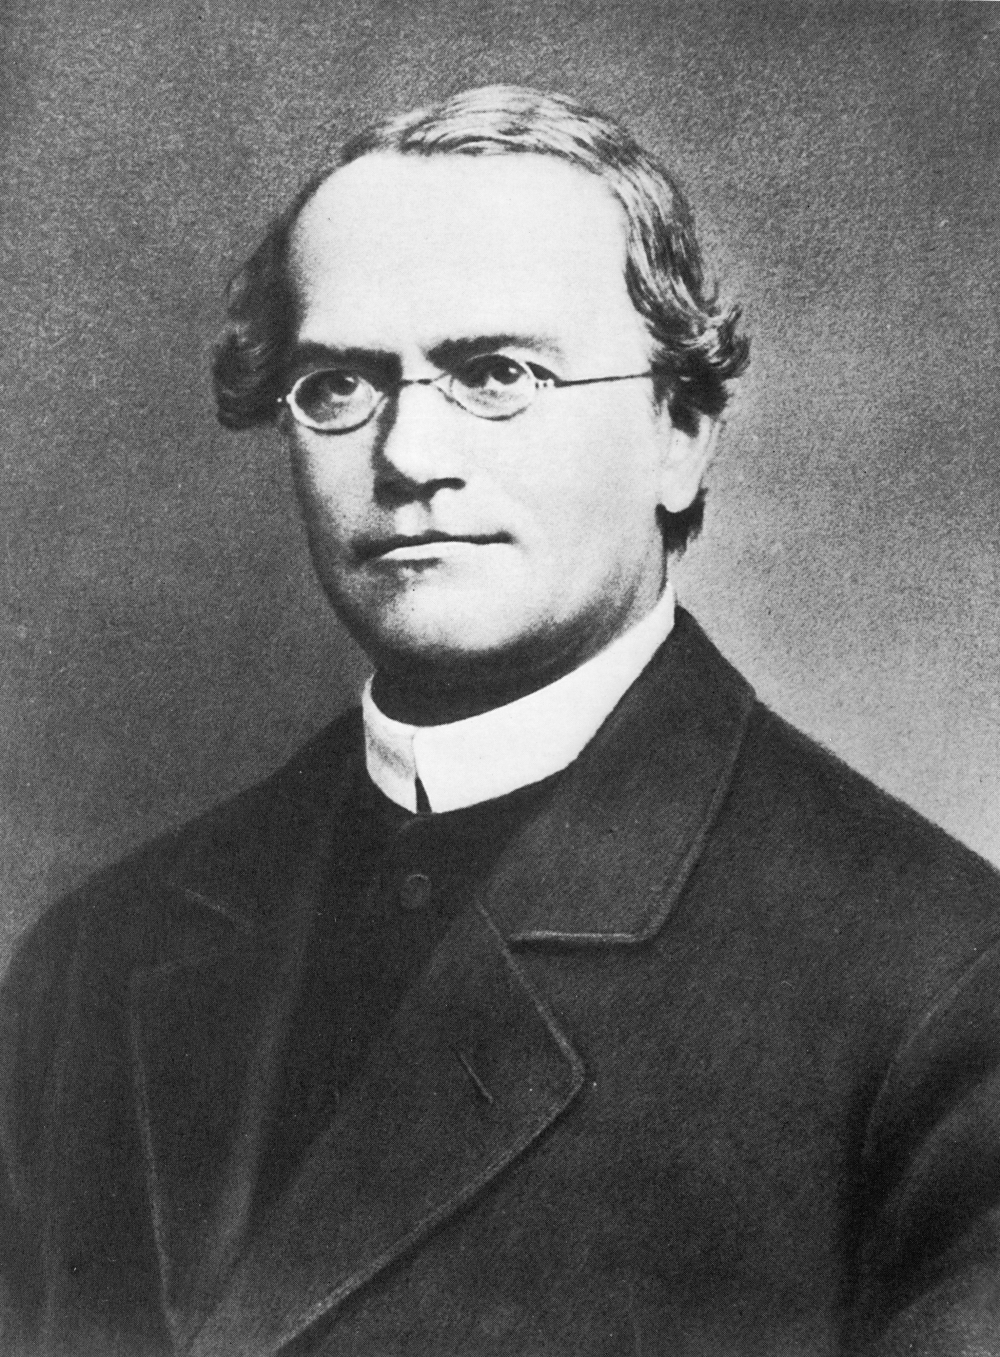
\includegraphics[width=0.3\linewidth]{images/book2/mendel.jpg}

{\small Gregor Mendel, que contou os descendentes de cruzamentos de ervilhas no jardim de um mosteiro nos anos 1860 e encontrou as proporções --- 3:1 para uma característica, 9:3:3:1 para duas --- que a \omterm{def:g12:meiosis-genetic-shuffling:meiosis}{meiose}, desconhecida dele, produz. Fotografia, domínio público.}
\end{omfigure}

\begin{method}[O cruzamento-teste]\label{met:g12:meiosis-genetic-shuffling:testcross}
Para ver que gametas um indivíduo fabrica, cruze-o com um parceiro que
carregue apenas \omterm{def:g10:universal-dna:gene}{alelos} \omterm{def:g11:genes-and-disease:genetic}{recessivos} (um \emph{cruzamento-teste}): cada
descendente mostra então exatamente os \omterm{def:g10:universal-dna:gene}{alelos} que o gameta do genitor
testado carregava. Para dois \omterm{def:g10:universal-dna:gene}{genes}, com o genitor testado $AaBb$ e o
parceiro $aabb$:
\begin{enumerate}
  \item Conte os quatro tipos de descendentes: $AB$, $Ab$, $aB$, $ab$
        (cada um carregando também $ab$ do parceiro).
  \item Se os quatro forem igualmente frequentes ($1:1:1:1$), os \omterm{def:g10:universal-dna:gene}{genes}
        estão em \omterm{def:g10:universal-dna:information}{cromossomos} diferentes e se segregam de modo
        independente.
  \item Se dois tipos (as combinações parentais) forem muito mais
        comuns que os outros dois (os recombinantes), os \omterm{def:g10:universal-dna:gene}{genes} estão no
        mesmo \omterm{def:g11:cell-cycle-mitosis:chromosome}{cromossomo}; os recombinantes vêm de uma \omterm{prop:g12:meiosis-genetic-shuffling:crossingover}{permutação}, e a
        proporção deles mede a distância entre os \omterm{def:g10:universal-dna:gene}{genes}.
  \item Os recombinantes são sempre a minoria e vêm sempre em duas
        classes iguais; o mesmo vale para os parentais.
\end{enumerate}
\end{method}

\begin{example}[Dois cruzamentos na mosca-das-frutas]\label{ex:g12:meiosis-genetic-shuffling:fly}
Mosca A, heterozigótica para a cor do corpo e a forma da asa, submetida
a um cruzamento-teste: 254 cinza-normais, 248 pretas-vestigiais, 251
cinza-vestigiais, 247 pretas-normais --- quatro classes iguais, os
\omterm{def:g10:universal-dna:gene}{genes} estão em \omterm{def:g10:universal-dna:information}{cromossomos} diferentes. Mosca B, heterozigótica para a
cor do corpo e a cor dos olhos: 412 cinza-vermelhas, 405
pretas-púrpuras, 44 cinza-púrpuras, 39 pretas-vermelhas --- duas
classes parentais de cerca de 45\% cada e duas classes recombinantes de
cerca de 5\%: os \omterm{def:g10:universal-dna:gene}{genes} estão no mesmo \omterm{def:g11:cell-cycle-mitosis:chromosome}{cromossomo}, perto um do outro,
separados por uma \omterm{prop:g12:meiosis-genetic-shuffling:crossingover}{permutação} em 9\% das \omterm{def:g12:meiosis-genetic-shuffling:meiosis}{meioses}.
\end{example}

\begin{omfigure}
\begin{tikzpicture}[font=\small]
  \draw[thick] (0,0) grid[step=1.4] (5.6,1.4);
  \node[fill=omDef!15, minimum width=1.3cm, minimum height=1.3cm, align=center] at (0.7,0.7) {$AB$\\ 254};
  \node[fill=omDef!15, minimum width=1.3cm, minimum height=1.3cm, align=center] at (2.1,0.7) {$Ab$\\ 251};
  \node[fill=omDef!15, minimum width=1.3cm, minimum height=1.3cm, align=center] at (3.5,0.7) {$aB$\\ 247};
  \node[fill=omDef!15, minimum width=1.3cm, minimum height=1.3cm, align=center] at (4.9,0.7) {$ab$\\ 248};
  \node[anchor=south] at (2.8,1.5) {mosca A: genes independentes, $1:1:1:1$};
  \begin{scope}[xshift=7.4cm]
    \draw[thick] (0,0) grid[step=1.4] (5.6,1.4);
    \node[fill=omProp!25, minimum width=1.3cm, minimum height=1.3cm, align=center] at (0.7,0.7) {$AB$\\ 412};
    \node[fill=omThm!20, minimum width=1.3cm, minimum height=1.3cm, align=center] at (2.1,0.7) {$Ab$\\ 44};
    \node[fill=omThm!20, minimum width=1.3cm, minimum height=1.3cm, align=center] at (3.5,0.7) {$aB$\\ 39};
    \node[fill=omProp!25, minimum width=1.3cm, minimum height=1.3cm, align=center] at (4.9,0.7) {$ab$\\ 405};
    \node[anchor=south] at (2.8,1.5) {mosca B: genes ligados, parentais $\gg$ recombinantes};
  \end{scope}
\end{tikzpicture}

{\small Os gametas de duas moscas heterozigóticas, lidos em
cruzamentos-teste. Classes iguais querem dizer segregação
independente; duas classes grandes e duas pequenas querem dizer que os
\omterm{def:g10:universal-dna:gene}{genes} estão ligados, com as classes pequenas produzidas por \omterm{prop:g12:meiosis-genetic-shuffling:crossingover}{permutação}.}
\end{omfigure}

\section{Quando o embaralhamento dá errado}

\begin{proposition}[Erros da meiose]\label{prop:g12:meiosis-genetic-shuffling:errors}
De vez em quando um par de homólogos não consegue se separar na \omterm{def:g12:meiosis-genetic-shuffling:meiosis}{meiose}
I, ou duas \omterm{def:g11:cell-cycle-mitosis:chromosome}{cromátides} na \omterm{def:g12:meiosis-genetic-shuffling:meiosis}{meiose} II: um gameta recebe duas cópias de um
\omterm{def:g11:cell-cycle-mitosis:chromosome}{cromossomo} e outro nenhuma. Fecundados, eles dão um zigoto com três
cópias (uma \emph{trissomia}) ou com uma (uma \emph{monossomia}). A
maioria desses zigotos não se desenvolve; os que se desenvolvem
carregam um conjunto de traços característicos. A trissomia do 21
(cerca de um nascimento em 700) causa deficiência intelectual e
defeitos cardíacos e é a mais comum; a frequência dela sobe
abruptamente com a idade da mãe. Uma \omterm{prop:g12:meiosis-genetic-shuffling:crossingover}{permutação} desigual --- \omterm{def:g11:cell-cycle-mitosis:chromosome}{cromátides}
trocando segmentos desiguais --- produz um \omterm{def:g11:cell-cycle-mitosis:chromosome}{cromossomo} com um \omterm{def:g10:universal-dna:gene}{gene}
duplicado e outro com uma deleção: o mecanismo pelo qual os \omterm{def:g10:universal-dna:gene}{genes} das
\omterm{def:g11:the-eye:photoreceptors}{opsinas} do \cref{ch:g11:the-eye} foram multiplicados, e pelo qual \omterm{def:g10:universal-dna:gene}{genes}
novos surgem (\cref{ch:g12:diversification-of-life}).
\end{proposition}
\admitted

\begin{omfigure}
\begin{tikzpicture}
\begin{axis}[
  width=0.84\linewidth, height=5.4cm,
  axis x line=bottom, axis y line=left,
  xmin=18, xmax=47, ymin=0, ymax=40,
  xlabel={idade da mãe (anos)}, ylabel={trissomia do 21 por 1000 nascimentos},
  xlabel style={font=\small, at={(axis description cs:0.5,-0.12)}, anchor=north},
  ylabel style={font=\small},
  tick label style={font=\small}, xtick={20,25,30,35,40,45}, ytick={0,10,20,30,40},
]
\addplot[thick, omThm, mark=*, mark size=1.5pt] coordinates
  {(20,0.7) (25,0.8) (30,1.1) (33,1.8) (35,2.9) (37,4.5) (39,7.5) (41,12) (43,20) (45,33)};
\end{axis}
\end{tikzpicture}

{\small Frequência da trissomia do 21 ao nascer em função da idade da
mãe. Os óvulos são formados antes do nascimento de uma mulher e ficam
pausados na \omterm{def:g12:meiosis-genetic-shuffling:meiosis}{meiose} I por décadas; quanto mais longa a pausa, mais
provável uma falha na separação dos homólogos.}
\end{omfigure}

\begin{example}[Cromossomos sexuais mal contados]\label{ex:g12:meiosis-genetic-shuffling:sexchrom}
Um gameta sem nenhum \omterm{def:g11:cell-cycle-mitosis:chromosome}{cromossomo} sexual fecundado por outro que carregue
um X dá um zigoto XO: uma menina de baixa estatura cujos ovários não se
desenvolvem. Um óvulo XX fecundado por um espermatozoide Y dá XXY: um
menino cujos testículos continuam pequenos e não fabricam
espermatozoides. Nos dois casos o \omterm{prop:g11:becoming-male-female:sry}{SRY} decide a gônada como no
\cref{ch:g11:becoming-male-female}; o número de \omterm{def:g10:universal-dna:information}{cromossomos} X decide
boa parte do resto, e é por isso que esses são os mais brandos dos
erros cromossômicos.
\end{example}

\begin{remark}[Por que sexo]\label{rem:g12:meiosis-genetic-shuffling:whysex}
Uma bactéria copia a si mesma; uma roseira pode crescer de uma estaca.
A reprodução sexuada é mais cara --- dois genitores, a \omterm{def:g12:meiosis-genetic-shuffling:meiosis}{meiose}, a busca
por um parceiro --- e o produto dela é um conjunto de descendentes cada
um diferente dos genitores e dos irmãos. Essa diferença é o ponto: num
ambiente que muda, e contra parasitas que evoluem, uma população de
indivíduos variados tem mais chance de conter alguns que sobrevivam do
que uma população de cópias. O embaralhamento deste capítulo é a
matéria-prima que a seleção dos dois capítulos seguintes vai separar.
\end{remark}

\section{Exercícios}

\begin{exercise}[$\star$]\label{exo:g12:meiosis-genetic-shuffling:1}
Defina \omterm{def:g12:meiosis-genetic-shuffling:meiosis}{diploide} e \omterm{def:g12:meiosis-genetic-shuffling:meiosis}{haploide}, e diga o que a \omterm{def:g12:meiosis-genetic-shuffling:meiosis}{meiose} faz com o número de
\omterm{def:g10:universal-dna:information}{cromossomos} e com a quantidade de \omterm{def:g10:universal-dna:information}{DNA}.
\end{exercise}

\begin{exercise}[$\star$]\label{exo:g12:meiosis-genetic-shuffling:2}
O que se separa na \omterm{def:g12:meiosis-genetic-shuffling:meiosis}{meiose} I? E na \omterm{def:g12:meiosis-genetic-shuffling:meiosis}{meiose} II? Qual das divisões é a
reducional?
\end{exercise}

\begin{exercise}[$\star$]\label{exo:g12:meiosis-genetic-shuffling:3}
Uma \omterm{def:g10:cells-common-unit:cell}{célula} tem $2n = 8$ e \omterm{def:g10:universal-dna:information}{DNA} $2q$ no início da \omterm{def:g12:meiosis-genetic-shuffling:meiosis}{meiose}. Dê o número de
\omterm{def:g10:universal-dna:information}{cromossomos} e a quantidade de \omterm{def:g10:universal-dna:information}{DNA} das \omterm{def:g10:cells-common-unit:cell}{células} depois da \omterm{def:g12:meiosis-genetic-shuffling:meiosis}{meiose} I e
depois da \omterm{def:g12:meiosis-genetic-shuffling:meiosis}{meiose} II.
\end{exercise}

\begin{exercise}[$\star$]\label{exo:g12:meiosis-genetic-shuffling:4}
Quantas combinações de \omterm{def:g10:universal-dna:information}{cromossomos} os gametas de uma \omterm{def:g10:biodiversity-scales:species}{espécie} com
$2n = 8$ podem apresentar só pela segregação independente?
\end{exercise}

\begin{exercise}[$\star$]\label{exo:g12:meiosis-genetic-shuffling:5}
O que é um cruzamento-teste, e o que a proporção de descendentes
recombinantes revela?
\end{exercise}

\begin{exercise}[$\star\star$]\label{exo:g12:meiosis-genetic-shuffling:6}
A partir da figura do \omterm{def:g10:universal-dna:information}{DNA}, leia o \omterm{def:g10:universal-dna:information}{DNA} por \omterm{def:g10:cells-common-unit:cell}{célula} de uma \omterm{def:g10:cells-common-unit:cell}{célula} na
\omterm{def:g12:meiosis-genetic-shuffling:meiosis}{meiose} I, de uma \omterm{def:g10:cells-common-unit:cell}{célula} entre as duas divisões e de um gameta. Explique
por que não há fase S entre as divisões.
\end{exercise}

\begin{exercise}[$\star\star$]\label{exo:g12:meiosis-genetic-shuffling:7}
Um cruzamento-teste dá 300 $AB$, 298 $ab$, 302 $Ab$, 300 $aB$. Os \omterm{def:g10:universal-dna:gene}{genes}
estão ligados? Quais são os gametas do genitor?
\end{exercise}

\begin{exercise}[$\star\star$]\label{exo:g12:meiosis-genetic-shuffling:8}
Um cruzamento-teste dá 460 $AB$, 455 $ab$, 42 $Ab$, 43 $aB$. Os \omterm{def:g10:universal-dna:gene}{genes}
estão ligados? Que classes são recombinantes, e que fração elas formam?
\end{exercise}

\begin{exercise}[$\star\star$]\label{exo:g12:meiosis-genetic-shuffling:9}
Na figura da \omterm{prop:g12:meiosis-genetic-shuffling:crossingover}{permutação}, que dois gametas você obteria se a troca
acontecesse \emph{acima} dos dois \omterm{def:g10:universal-dna:gene}{genes}? Explique.
\end{exercise}

\begin{exercise}[$\star\star$]\label{exo:g12:meiosis-genetic-shuffling:10}
A partir da figura da trissomia, leia a frequência aos 25, aos 35 e aos
42 anos, e calcule o fator entre 25 e 42.
\end{exercise}

\begin{exercise}[$\star\star$]\label{exo:g12:meiosis-genetic-shuffling:11}
Explique como uma não disjunção na \omterm{def:g12:meiosis-genetic-shuffling:meiosis}{meiose} I difere de uma na \omterm{def:g12:meiosis-genetic-shuffling:meiosis}{meiose} II
quanto aos gametas produzidos (considere as quatro \omterm{def:g10:cells-common-unit:cell}{células}).
\end{exercise}

\begin{exercise}[$\star\star\star$]\label{exo:g12:meiosis-genetic-shuffling:12}
Dois \omterm{def:g10:universal-dna:gene}{genes} do mesmo \omterm{def:g11:cell-cycle-mitosis:chromosome}{cromossomo} recombinam em 2\% das \omterm{def:g12:meiosis-genetic-shuffling:meiosis}{meioses}; outros
dois do mesmo \omterm{def:g11:cell-cycle-mitosis:chromosome}{cromossomo}, em 48\%. Explique o que cada número diz sobre
a distância entre eles, e por que o segundo par se comporta quase como
\omterm{def:g10:universal-dna:gene}{genes} independentes.
\end{exercise}

\begin{exercise}[$\star\star\star$]\label{exo:g12:meiosis-genetic-shuffling:13}
Uma planta tem $2n = 4$, um par carregando $A/a$ e o outro $B/b$.
Liste todos os gametas de uma planta $AaBb$ com as frequências deles,
sem \omterm{prop:g12:meiosis-genetic-shuffling:crossingover}{permutação}; depois diga o que a \omterm{prop:g12:meiosis-genetic-shuffling:crossingover}{permutação} mudaria.
\end{exercise}

\begin{exercise}[$\star\star\star$]\label{exo:g12:meiosis-genetic-shuffling:14}
Gêmeos idênticos compartilham todos os \omterm{def:g10:universal-dna:gene}{alelos}; irmãos comuns
compartilham metade, em média. Explique essa ``metade'' com a \omterm{def:g12:meiosis-genetic-shuffling:meiosis}{meiose} e
a fecundação, e por que ela é uma média.
\end{exercise}

\begin{exercise}[$\star\star\star$]\label{exo:g12:meiosis-genetic-shuffling:15}
Algumas plantas se reproduzem por sementes formadas sem \omterm{def:g12:meiosis-genetic-shuffling:meiosis}{meiose} nem
fecundação. Explique o que são geneticamente os descendentes delas, o
que uma planta dessas ganha, e o que ela perde a longo prazo.
\end{exercise}

\section{Problema: as moscas do geneticista}

\begin{problem}[{Problema de fim de semana --- dois genes acompanhados
pela meiose e por um cruzamento-teste: os gametas contados, a ligação
decidida, a recombinação medida, e o número de mãos que um casal
consegue distribuir}]
\label{pb:g12:meiosis-genetic-shuffling:1}
Na mosca-das-frutas, o \omterm{def:g10:universal-dna:gene}{alelo} $b$ (corpo preto) é \omterm{def:g11:genes-and-disease:genetic}{recessivo} em relação a
$b^+$ (cinza), e $vg$ (asas vestigiais) é \omterm{def:g11:genes-and-disease:genetic}{recessivo} em relação a $vg^+$
(normais). Uma fêmea cinza de asas normais, cujos pais eram cinza-normais
puros e pretos-vestigiais puros, é cruzada com um macho preto de asas
vestigiais. Descendentes: cinza-normais 965, pretos-vestigiais 944,
cinza-vestigiais 206, pretos-normais 185.

\medskip
\noindent\textbf{Parte I --- O cruzamento.}
\begin{enumerate}
  \item Dê o \omterm{def:g11:enzymes-and-phenotype:phenotype}{genótipo} da fêmea e o do macho, \omterm{def:g10:universal-dna:gene}{gene} por \omterm{def:g10:universal-dna:gene}{gene}.
  \item Que gametas o macho produz? Por que isso faz do cruzamento um
        cruzamento-teste?
  \item Liste os quatro gametas que a fêmea poderia produzir, e os
        descendentes que cada um dá.
  \item Calcule a porcentagem de cada classe entre os 2300
        descendentes.
  \item Os dois \omterm{def:g10:universal-dna:gene}{genes} estão no mesmo \omterm{def:g11:cell-cycle-mitosis:chromosome}{cromossomo} ou em \omterm{def:g10:universal-dna:information}{cromossomos}
        diferentes? Justifique pelas proporções.
\end{enumerate}

\medskip
\noindent\textbf{Parte II --- Dentro da \omterm{def:g12:meiosis-genetic-shuffling:meiosis}{meiose} da fêmea.}
\begin{enumerate}[resume]
  \item Que duas classes são as combinações parentais, e de onde elas
        vêm nos \omterm{def:g10:universal-dna:information}{cromossomos} da fêmea?
  \item Que duas são recombinantes? Por que evento da \omterm{def:g12:meiosis-genetic-shuffling:meiosis}{meiose} I elas
        surgiram?
  \item Calcule a frequência de recombinação (recombinantes sobre o
        total). Em que fração das \omterm{def:g12:meiosis-genetic-shuffling:meiosis}{meioses} da fêmea houve uma \omterm{prop:g12:meiosis-genetic-shuffling:crossingover}{permutação}
        entre os dois \omterm{def:g10:universal-dna:gene}{genes}?
  \item Explique por que as duas classes recombinantes são quase
        iguais, e por que as duas classes parentais também são.
  \item Os mesmos dois \omterm{def:g10:universal-dna:gene}{genes}, numa fêmea cujos pais eram
        cinza-vestigiais puros e pretos-normais puros: preveja as
        quatro classes e as frequências delas.
\end{enumerate}

\medskip
\noindent\textbf{Parte III --- Um terceiro \omterm{def:g10:universal-dna:gene}{gene}.}
Um terceiro \omterm{def:g10:universal-dna:gene}{gene}, $cn$ (olhos cinábrio), é submetido a um
cruzamento-teste com $b$ em outra fêmea: 9\% de recombinantes. Com
$vg$: 8\% de recombinantes.
\begin{enumerate}[resume]
  \item O $cn$ está no mesmo \omterm{def:g11:cell-cycle-mitosis:chromosome}{cromossomo} que $b$ e $vg$?
  \item Usando as três frequências de recombinação (17\% para
        $b$--$vg$, 9\% para $b$--$cn$, 8\% para $cn$--$vg$), coloque os
        três \omterm{def:g10:universal-dna:gene}{genes} em ordem ao longo do \omterm{def:g11:cell-cycle-mitosis:chromosome}{cromossomo}.
  \item Explique por que as frequências se somam (quase), e o que isso
        diz sobre a relação entre recombinação e distância.
  \item Dois \omterm{def:g10:universal-dna:gene}{genes} nas extremidades opostas de um \omterm{def:g11:cell-cycle-mitosis:chromosome}{cromossomo} comprido
        dão 50\% de recombinantes. Explique por que a frequência não
        pode passar de 50\%.
  \item Um quarto \omterm{def:g10:universal-dna:gene}{gene} dá 50\% de recombinantes com os três. O que você
        pode concluir, e o que você não pode?
\end{enumerate}

\medskip
\noindent\textbf{Parte IV --- O tamanho do baralho.}
A mosca-das-frutas tem $2n = 8$.
\begin{enumerate}[resume]
  \item Quantas combinações de \omterm{def:g10:universal-dna:information}{cromossomos} os gametas de uma mosca
        podem apresentar só pela segregação independente? E os
        descendentes de um casal de moscas?
  \item Com uma \omterm{prop:g12:meiosis-genetic-shuffling:crossingover}{permutação} em posição variável em cada par, explique
        por que o número de gametas distintos fica praticamente
        ilimitado.
  \item Para um casal humano, calcule o número de combinações de
        \omterm{def:g10:universal-dna:information}{cromossomos} dos filhos deles só pela segregação, e compare com
        o número de seres humanos que já viveram (cerca de $10^{11}$).
  \item Explique por que dois irmãos são, ainda assim, mais parecidos
        entre si do que dois estranhos, em termos dos \omterm{def:g10:universal-dna:gene}{alelos} que eles
        podem ter recebido.
  \item Enuncie o resultado: a frequência de recombinação entre $b$ e
        $vg$, o que ela mede, e os dois mecanismos da \omterm{def:g12:meiosis-genetic-shuffling:meiosis}{meiose} que fazem
        cada gameta da fêmea ser diferente.
\end{enumerate}
\end{problem}
